\documentclass[../../report.tex]{subfiles}
\begin{document}
\section{Artificial Neural Networks}

The past decade has seen rapid advancement in a class of techniques commonly
known as \emph{deep learning}. The core idea is simple -- stacking several
layers of simple, but nonlinear modules creates a computational network that, as
a whole, can approximate very complex functions. Through successive optimisation
rounds of the layered modules' parameters, the network can be nudged towards a
specific goal. Ideally, after many iterations of optimisation, the network
converges to that goal.

Previously, machine learning tasks required a lot of manual work and specialised
knowledge in order to transform task-specific data into a representation that
made the task tractable. The key innovation of deep learning is automated
feature extraction, most usefully from complex, high dimensional input data,
e.g. images. In classification tasks, it is particularly desirable that the
feature extractor transforms the intractable input space into a space where
inputs belonging to different classes are \emph{linearly separable} (figure
\ref{fig:representation-learning}). \cite{LeCun2015}

\begin{figure}
  \centering
  \begin{subfigure}[b]{0.49\textwidth}
    \centering
    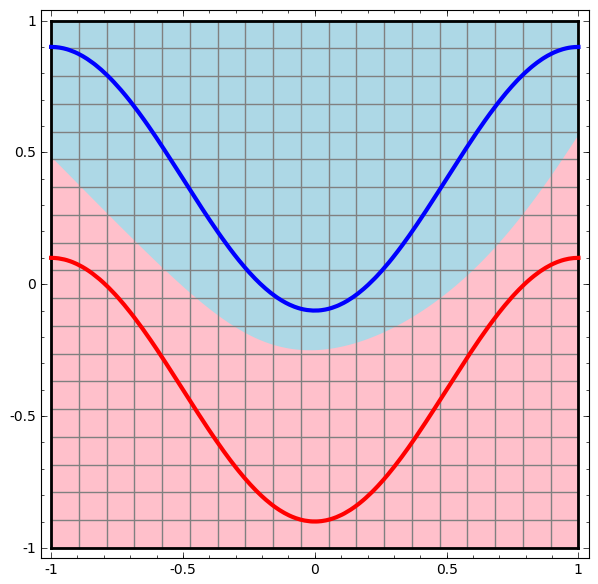
\includegraphics[width=0.75\textwidth]{boundary-nonlinear}
    \caption{Input space}
  \end{subfigure}
  \hfill
  \begin{subfigure}[b]{0.49\textwidth}
    \centering
    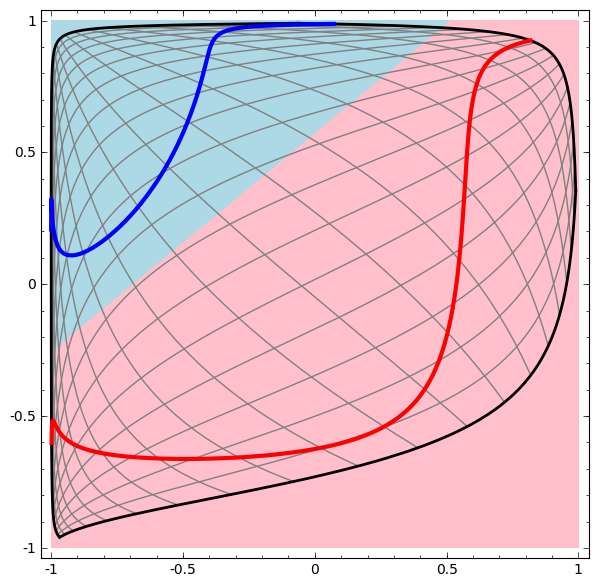
\includegraphics[width=0.75\textwidth]{boundary-linear}
    \caption{Learned representation}
  \end{subfigure}
  \caption{The network learns to separate nonlinear data. \cite{Olah2014}}
  \label{fig:representation-learning}
\end{figure}

\subsection{Feedforward networks}

As introduced above, these powerful feature extractors consist of several
layers. First, there is the input layer, which is filled with input data prior
to the computation. This data then flows through zero or more hidden layers,
before finally finding its way to the output layer (figure
\ref{fig:feedforward}). The \emph{activation} of each unit in every non-input
layer is given by a weighted sum over all activations of the previous layer.
This sum is finally taken through a nonlinear function, e.g.
ReLU\footnote{Rectified Linear Unit}, which is simply \(f(x) = max(0, x)\).

\begin{figure}
  \centering
  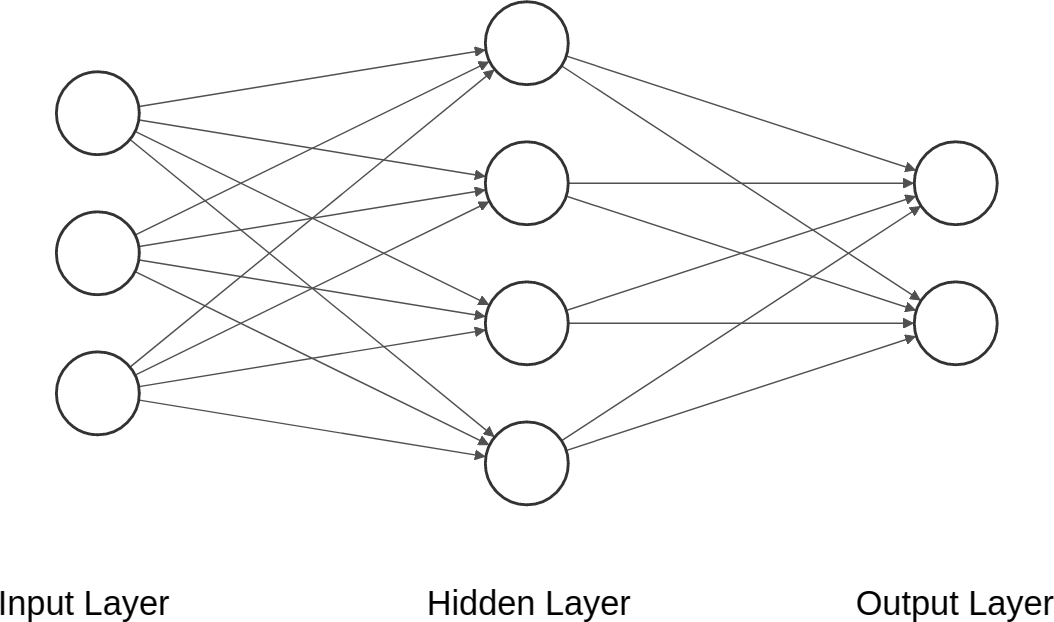
\includegraphics[width=0.75\textwidth]{feedforward}
  \caption{Feedforward network.}
  \label{fig:feedforward}
\end{figure}

\subsubsection{Backpropagation}
To unlock the full potential of these networks, it is imperative to optimise the
weights determining the activation of individual units. To do so, a \emph{loss
function} is required. Figuratively, this is a measure of distance between the
network's output and the ground truth value. Clearly, this distance should be
minimised. This is achieved with the help of calculus, namely \emph{partial
derivatives} and the \emph{chain rule}. Loosely speaking, a partial derivative
quantifies a given variable's influence towards a multivariate function; the
chain rule allows calculating such partial derivatives even when the variable in
question is hidden behind several layers of function composition. Crucially,
this forms the foundation for backpropagation, a procedure that computes the
influence towards the loss function for every network parameter \emph{in
isolation} (figure \ref{fig:backpropagation}).

\subsubsection{Gradient descent}
Once calculated, the error contributions of individual parameters can be
combined into a \emph{gradient}, which in a sense describes the direction of
steepest increase\footnotemark{} for the loss function. Of course, as this
function is subject to minimisation, the relevant step is in the direction
exactly opposite of the gradient. This simple idea is known as gradient descent,
and it represents the `nudge' introduced at the beginning of this section.

\footnotetext{A good visual analogy is that of hill-climbing, although this
quickly breaks down, as neural network gradients are usually in high-dimensional
space.}

\begin{figure}
  \centering
  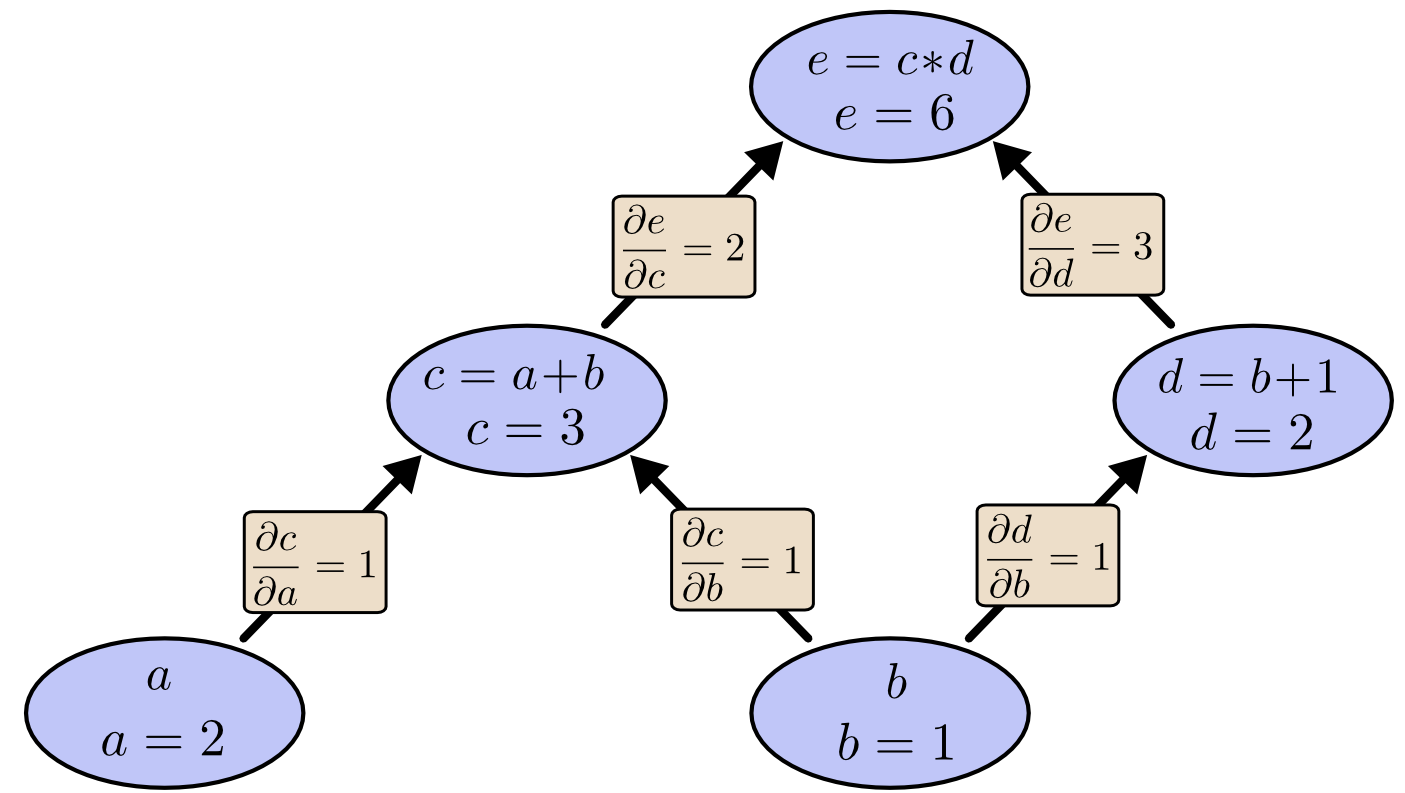
\includegraphics[width=0.75\textwidth]{backpropagation}
  \caption{Backpropagation in a computational graph. \cite{Olah2015Backprop}}
  \label{fig:backpropagation}
\end{figure}

\subsection{Recurrent networks}

Although feedforward networks are undoubtedly powerful, they are not very well
suited for processing sequential data. This is partially because they require
fixed-size inputs, whereas sequences usually vary in length. This is certainly a
problem for a generative music model, which should be able to process both short
and long melodies. Recurrent neural networks (RNNs) account for this deficiency
by processing sequences one step at a time, while maintaining an \emph{internal
state} that encodes information about previous inputs. At each step, the
previous state is used in combination with the input to produce the next state
(figure \ref{fig:rnn-unrolled}). This is quite different from a feedforward
network, whose output depends purely on the current input.

\subsubsection{Backpropagation through time}
The optimisation procedure for recurrent networks is similar to that of
feedforward networks. If we unfold the RNN across time steps, the result is
essentially a feedforward network with many\footnotemark{} hidden layers (figure
\ref{fig:rnn-unrolled}). Only this time, all layers share the same parameters,
and the input and output layers are `spread' across the hidden layers, i.e.
time. Performing backpropagation on this unfolded version of the RNN is known as
backpropagation through time, or BPTT.

\footnotetext{In fact, the number of layers is equal to the length of the input
sequence.}

\begin{figure}
  \centering
  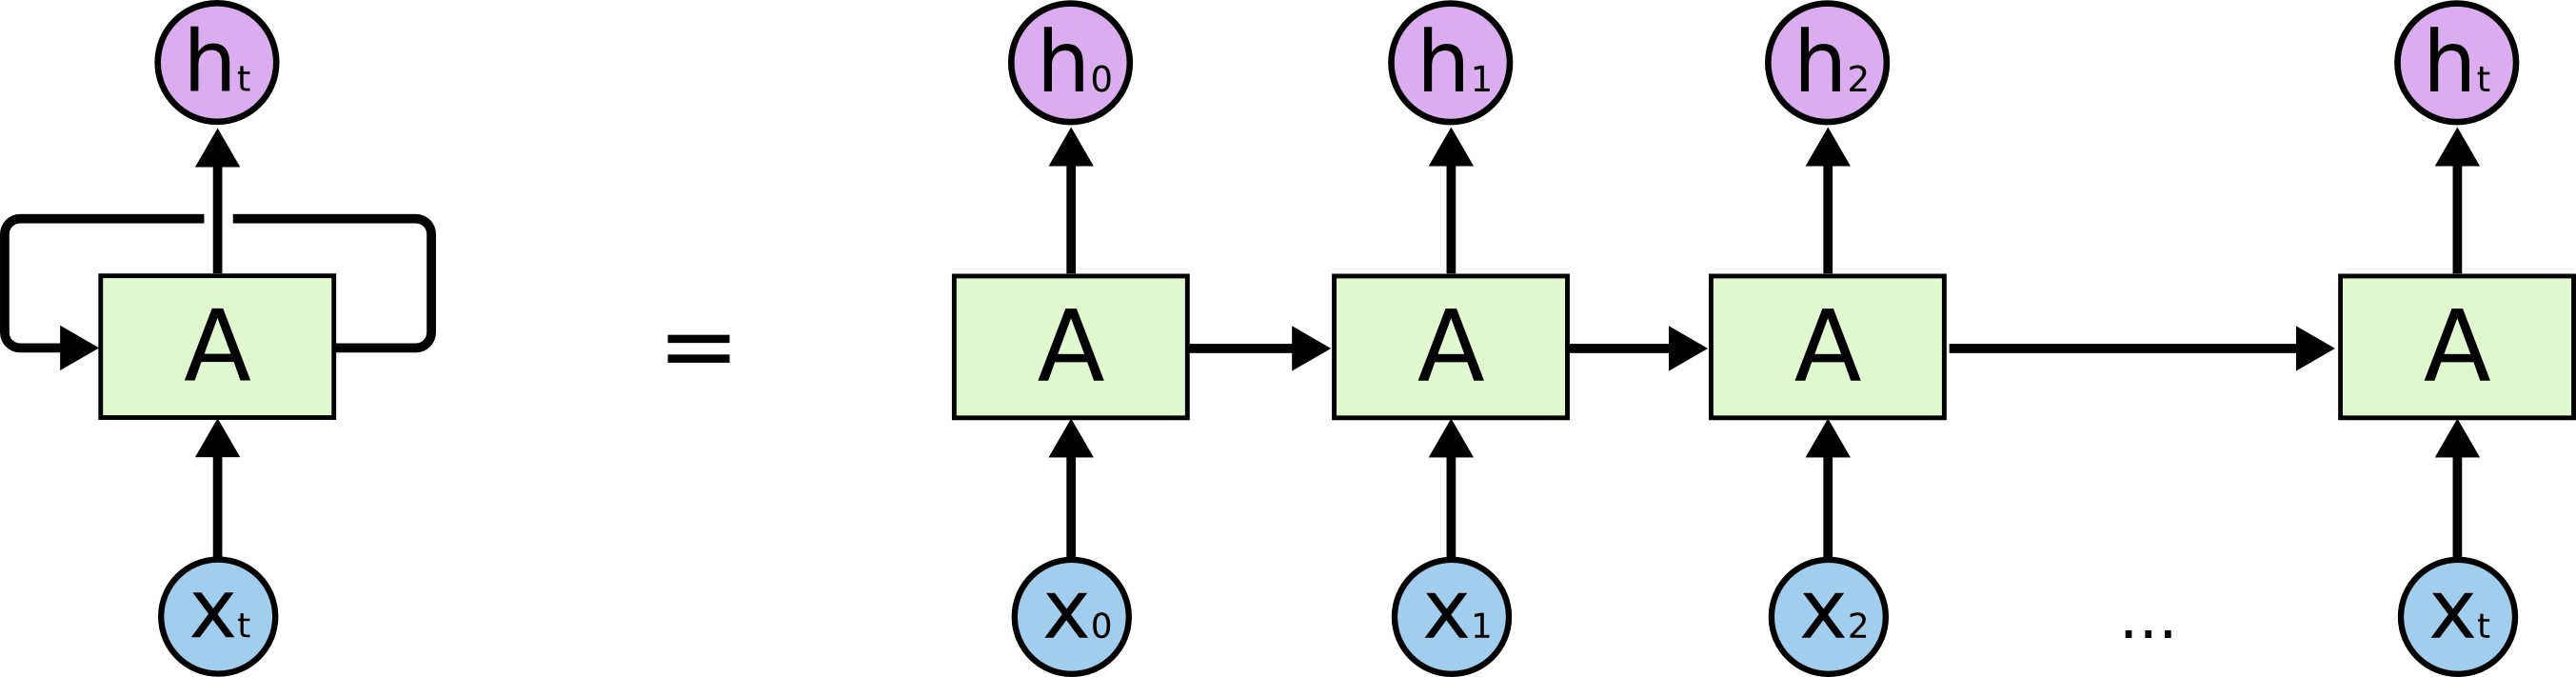
\includegraphics[width=\textwidth]{rnn-unrolled}
  \caption{Input \(x_t\) is used to produce new states \(h_t\). The RNN cell
  (left) is unrolled across time for training (right). \cite{Olah2015LSTM}}
  \label{fig:rnn-unrolled}
\end{figure}

\subsubsection{Long Short-Term Memory}
The idea of using RNNs to model long-term temporal dependencies is appealing,
however it has been shown \cite{Bengio1994} that in practice, it is difficult
for RNNs to remember relevant past inputs for a long time. Instead it is common
to use Long Short-Term Memory (LSTM) networks \cite{Hochreiter1997}. Their key
innovation is explicit modelling of forgetting and accumulation of memory.
Whereas in RNNs the state is transformed by a single feedforward layer, the LSTM
employs four -- each with a specific purpose (figure \ref{fig:lstm}). This makes
it very easy for LSTMs to retain parts of the previous state, which in turn
captures long-term dependencies.

\begin{figure}
  \centering
  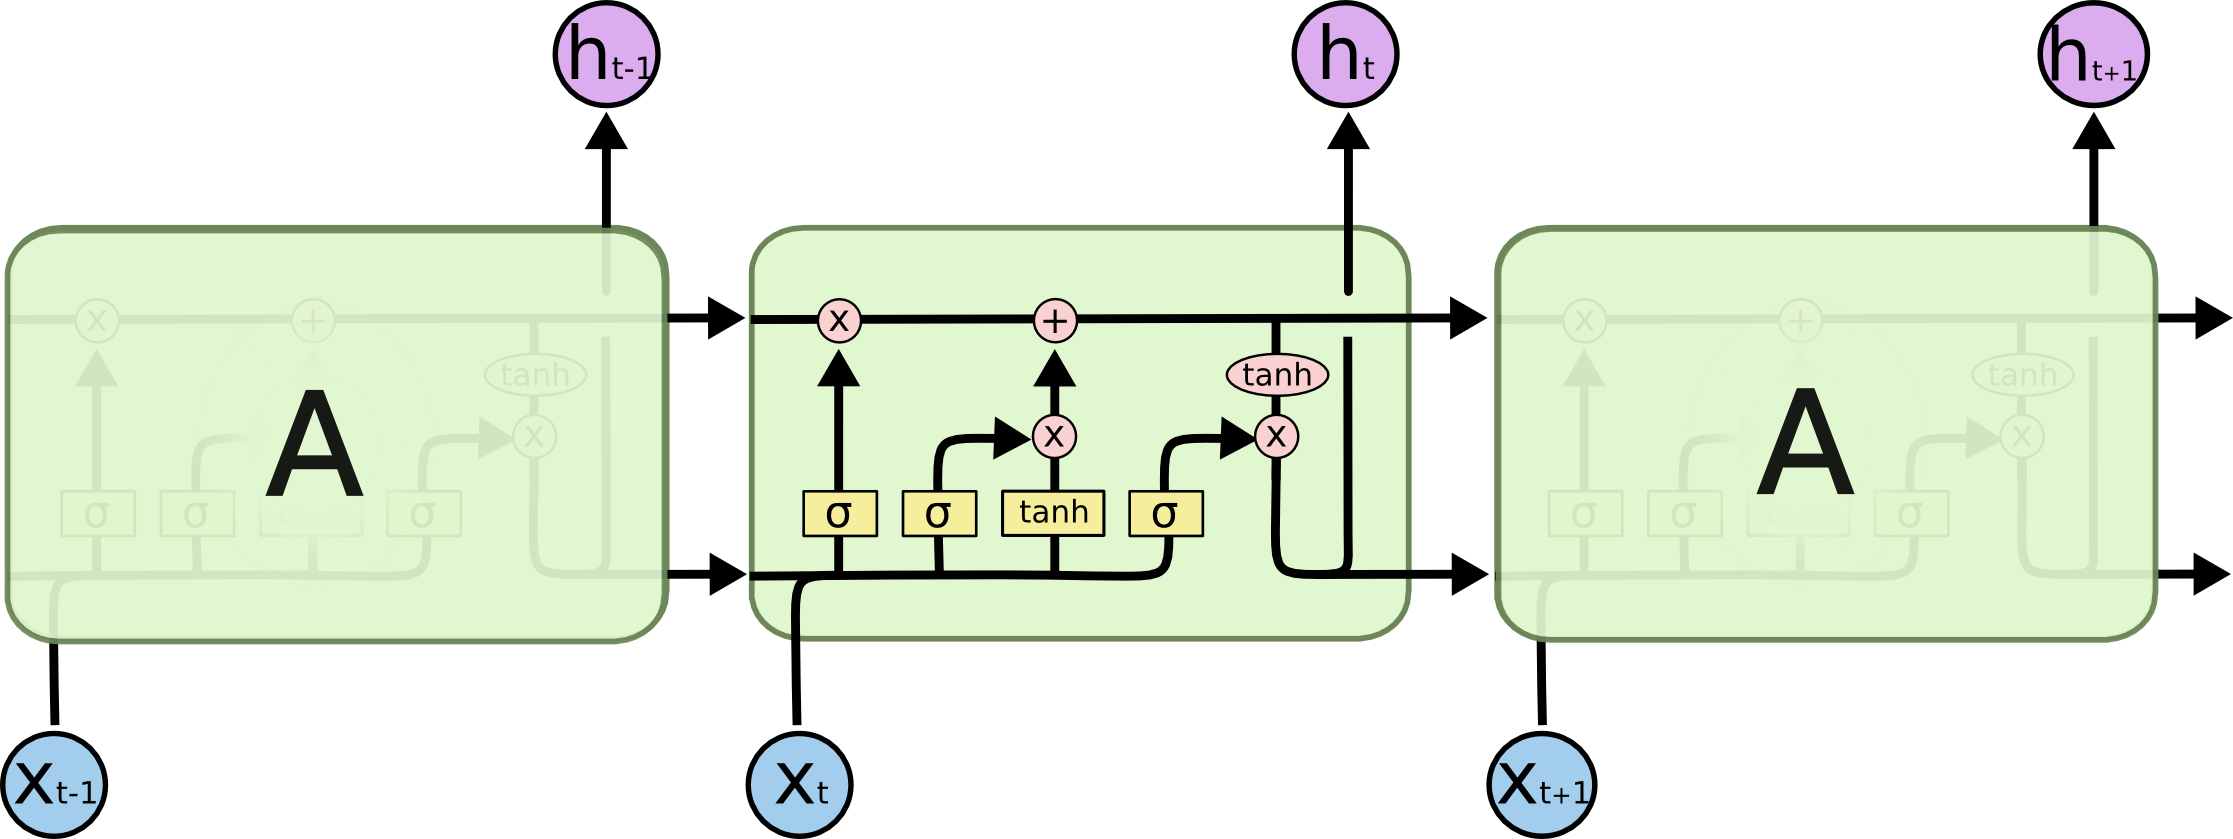
\includegraphics[width=\textwidth]{lstm}
  \caption{An LSTM cell contains multiple gates for state manipulation. \cite{Olah2015LSTM}}
  \label{fig:lstm}
\end{figure}

\end{document}
